\section{Simulations}

\subsection{Constant length pendulum}

In this first part, we will consider the case where \(\alpha=0\) and \(d=0\), that is the length of the pendulum remains constant \(\ell(t)=L\). This corresponds to the situation analysed in \autoref{sec:analytic:constant_length}. Using a small initial angle of \(\theta_0=10^{-10}\) and no initial speed, a convergence study of the final angle and angular speed of the Velocity Verlet method was done. Comparing the final position obtained numerically with the analytical result, we obtain an error on the final position. The results in \autoref{fig:numeric_convergence_small_angle} show that the order of convergence of this method, for these initial conditions, are 4 and 2 for the position and speed respectively.

\begin{figure}[h]
    \centering
    \begin{subfigure}{0.48\linewidth}
        \centering
        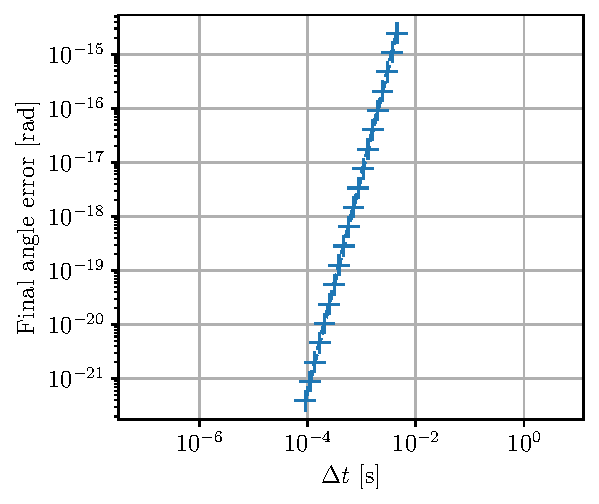
\includegraphics[width=\linewidth]{figures/no_excitation_pos_conv.pdf}
        \caption{Position (angle of pendulum)}
    \end{subfigure}
    \begin{subfigure}{0.48\linewidth}
        \centering
        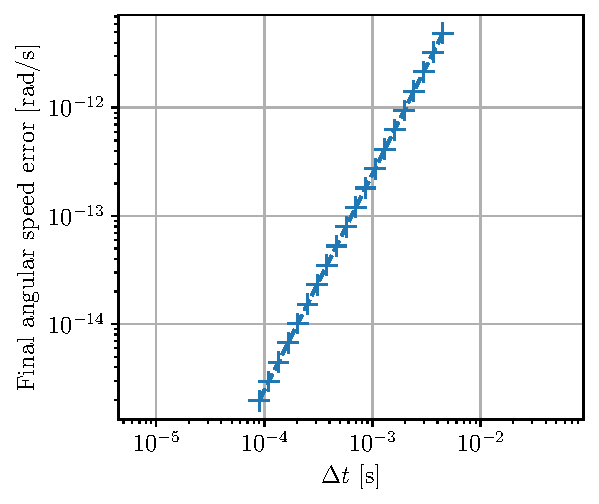
\includegraphics[width=\linewidth]{figures/no_excitation_vel_conv.pdf}
        \caption{Angular velocity}
    \end{subfigure}
    \caption{Numeric convergence of different variables for initial conditions \(\theta_0=10^{-10}\), \(\dot\theta_0=0\) and simulated until \(t_\textrm{fin} \approx 2.69\), corresponding to 3 periods of oscillation.}
    \label{fig:numeric_convergence_small_angle}
\end{figure}

Varying the initial angle \(\theta_0\) between \(0\) and \(\pi\) allows us to get larger motion of the pendulum, as shown in \autoref{fig:oscillations_time}. The angular frequency was extracted by looking at the time elapsed between the starting condition and the time it takes for two sign changes in angular speed (otherwise we would be mesuring a half-period). Writing that time as \(T\), the period of oscillation, we get the angular frequency \(\Omega = \frac{2\pi}{T}\). The results are shown in \autoref{fig:angular_frequency}. These results are coherent with the physical reality, as a larger angle should correspond to a longer oscillation period than a smaller angle. It is interesting to note that the angular frequency does not change linearly, which is consistent the results measured in the lab: small angles have less effect than large angles.

\begin{figure}[h]
    \centering
    \begin{subfigure}{0.48\linewidth}
        \centering
        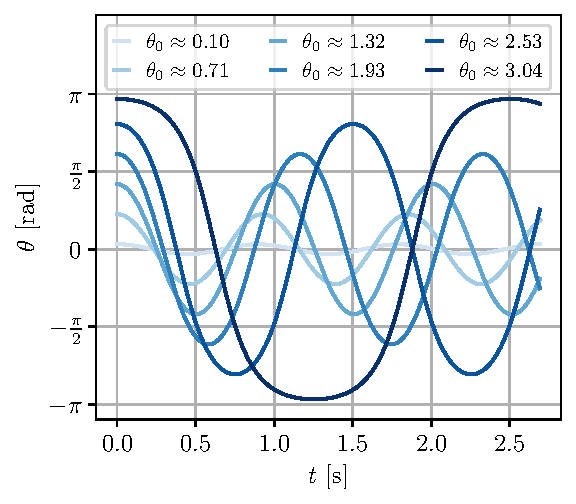
\includegraphics[width=\linewidth]{figures/oscillations_trajectory.pdf}
        \caption{Time evolution}
        \label{fig:oscillations_time}
    \end{subfigure}
    \begin{subfigure}{0.48\linewidth}
        \centering
        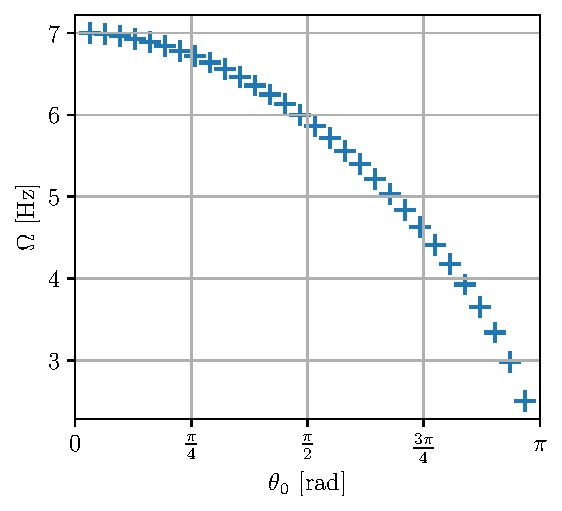
\includegraphics[width=\linewidth]{figures/angular_frequency.pdf}
        \caption{Angular frequency}
        \label{fig:angular_frequency}
    \end{subfigure}
    \caption{Time evolution and angular frequency for multiple starting angles (\(n_\textrm{steps}=10000\))}
\end{figure}

\subsection{Feur 1}

\subsection{Feur 2}

\subsection{Feur 3}
